% --- Style sheet setup ---
\documentclass[table]{style/USN-MSc}

% --- Bibliography setup ---
\usepackage[style=ieee, sorting=none]{biblatex}
\addbibresource{references.bib}

% --- Useful packages ---
\usepackage[
	photo={images/USN-cover-image.png}, % Optional
%    description={},% Optional
    %
    %
    %
   logo={images/USN-symbol_sort.pdf} % Defaults to a vectorized version of USN logo
%	author={\@author} % Sourced from \author command, can be set separately
%	title={\@title} % Sourced from \title command, can be be set separately
%	school={University of South-Eastern Norway}, % Default
%	faculty={Faculty of Technology and Maritime Sciences}, % Default
%	thesis={Master of Science thesis in Computer Science}, % Default
%	department={Department of Science and Industry Systems}, % Default
%	time={\@date}, % Sourced from \date command, can be set separately % Default is today's date
%	top=25mm, % Top margin
%	bottom=25mm, % Bottom margin
%	left=25mm, % Left Margin
%	right=25mm, % Right Margin
]{style/USN-frontpage}
\let\ordinal\relax  %fix for datetime package, see https://tex.stackexchange.com/questions/162353/memoir-class-conflict-with-datetime
\usepackage{datetime} % allow year and dates be displayed
\newdateformat{monthyeardate}{\monthname[\THEMONTH], \THEYEAR}
  
\usepackage{quotchap} % allow \begin{savequote} chapter start quotes 
\usepackage{tipa} % allow \textipa for phonetic symbols
\usepackage{diagbox} % allow the top left cell of a table to be split with a diagonal line
\usepackage{amssymb} % allow \varnothing for the empty set symbol
\usepackage{amsmath} % allow \fraq for fractions
\usepackage{hvfloat} % allow double page images that automatically split over two pages and has proper caption support
\usepackage[hypcap=false]{caption} 
\usepackage{siunitx} % allow \ohm for standard units like ohm symbol
\usepackage{float} % allow manual placement of images when automatic placement is poor
\usepackage{listings} %allow code listings
\usepackage[]{xcolor} 

\definecolor{USN-purple}{RGB}{70, 70, 165}
\definecolor{USN-green}{RGB}{34,150,138}
\definecolor{codegray}{rgb}{0.5,0.5,0.5}
\definecolor{backcolour}{rgb}{0.95,0.95,0.92}
\definecolor{MyTableCellColor}{RGB}{128, 128, 128}

\colorlet{chaptergrey}{USN-purple}

\lstdefinestyle{mystyle}{
    backgroundcolor=\color{backcolour},   
    commentstyle=\color{USN-green},
    keywordstyle=\color{USN-purple},
    numberstyle=\tiny\color{codegray},
    stringstyle=\color{USN-purple},
    basicstyle=\ttfamily\footnotesize,
    breakatwhitespace=false,         
    breaklines=true,                 
    captionpos=b,                    
    keepspaces=true,                 
    numbers=left,                    
    numbersep=5pt,                  
    showspaces=false,                
    showstringspaces=false,
    showtabs=false,                  
    tabsize=2
}

\lstset{style=mystyle}

\setcounter{secnumdepth}{2}
\setcounter{tocdepth}{2}


% --- Cover page ---
\newcommand{\mytitle}{%
%% title:
Thesis Title
}

\newcommand{\myauthor}{%
%% author:
First Last
}

\newcommand{\mykeywords}{%
%% keywords (used in the PDF document properties for indexing): see https://www.ieee.org/content/dam/ieee-org/ieee/web/org/pubs/ieee-taxonomy.pdf
<keyword 1, keyword 2, keyword 3 \ldots>
}



\begin{document}
%% Create cover page with image using parameters above
\USNfrontpage

%% Create copyright page using parameters above
\CopyRightPage

%% Create title page with the parameters given in the preamble above
\USNtitlepage

%% Add sections

%anothwr structure would be more topic oriented vs paper . Eg intro, mvl theory, RRAM programming incl DAC, Mixed Radix Circuit design, conxlusion
\pagenumbering{Roman}
~\\[10\baselineskip]

\begin{center}
\textit{Dedicated to ...}
\end{center}
\chapter*{Preface}
\label{sec:preface}
\addcontentsline{toc}{chapter}{Preface}
This dissertation is submitted in partial fulfilment of the requirements for the degree of Master of Science in Computer Science from the Department of Science and Industry Systems at the University of South-Eastern Norway (USN). The thesis work presented here took place between X and X. The work has been done under the supervision of Professor X and Y.

%possible ethics statement

%possible financial statement

%possible conflict of interest statement


\section*{Acknowledgements}
I would like to thank .. for ..

\textbf{\myauthor} \\
Kongsberg, January 2024
\chapter*{Abstract}
\label{sec:abstract}
\addcontentsline{toc}{chapter}{Abstract}


%improve keywords to get more hits
\textbf{Keywords:} keyword 1, keyword 2, keyword 3

%https://www.ieee.org/content/dam/ieee-org/ieee/web/org/pubs/ieee-taxonomy.pdf

%% table of contents
\tableofcontents
\addcontentsline{toc}{chapter}{\contentsname}

% comment out if unwanted
\chapter*{List of Papers}
\addcontentsline{toc}{section}{List of Papers}

\textbf{Article 1}
\newline
\textbf{F. Last}, C.O. Author "Paper A", \textit{2024 IEEE X}, Conference, Location, 2024, pp. 1-4, doi: ....

% comment out if unwanted
\listoffigures 
\addcontentsline{toc}{section}{\listfigurename}

% comment out if unwanted
\listoftables  
\addcontentsline{toc}{section}{\listtablename}

% comment out if unwated
\lstlistoflistings
\addcontentsline{toc}{section}{Code listings}

\chapter*{Nomenclature}
\addcontentsline{toc}{section}{Nomenclature}
\label{sec:nomenclature}

\begin{longtable}{ll}
  \textbf{Symbol} & \textbf{Explanation}\endhead\\
  ALU & Arithmethic Logic Unit \\
  ASIC & Application Specific Integrated Circuit \\
  VLSI & Very Large Scale Integration \\
\end{longtable}

%use thesaurus
%https://www.ieee.org/content/dam/ieee-org/ieee/web/org/pubs/ieee-thesaurus.pdf
\begin{savequote}
---"Famous Quote"
\qauthor{\textbf{Prof. Y}, in: \cite{RineMVLbook}}
\end{savequote}

\chapter{Introduction}
\label{ch:intro}
\pagenumbering{arabic}

\section{Various Overleaf examples}

\textbf{Example of a quote}
\begin{displayquote}
"This is a quote."
\end{displayquote}

\textbf{Example of an equation}
\begin{equation} \label{eq:1}
n = x_{p} * r^{p} + x_{p-1} * r^{p-1} + \dots + x_{0} * r^{0}
\end{equation}

\textbf{Example of a citation}
This topic is discussed in more detail with page number in \cite[p.~3]{BosBeyondCMOS}. The source code and results are made open source \cite{bos-mrcsGithub}. Example of a multi source: \cite{RineMVLbook,BosBeyondCMOS,bos-mrcsGithub}.

\textbf{Example of a footnote}
Note that this true in some cases\footnote{This is a footnote}. 

\textbf{Example of a bullet point list}
\begin{itemize}
    \item \textbf{Item 1.} Something
    \item \textbf{Item 2.} Another thing
    \item \textbf{Item 3.} More things?
\end{itemize}

\textbf{Example of a table}
\begin{table}[H]
\centering
\caption{Relation between discrete radixes, compactness and ambiguity}
\label{tab: radix-compactness}

\begin{tabular}{|c|cccc|}
 \hline
 \multicolumn{1}{|c|}{\textbf{Decimal Number}} &
 \multicolumn{4}{c|}{\textbf{Radix}} \cr \cline{2-5} 
  
 \multicolumn{1}{|c|}{\textbf{(Radix-10)}} &
 \multicolumn{1}{c}{\textbf{Radix-1}} & \textbf{Radix-2} & \cellcolor{USN-green!50}\textbf{Radix-3} & \textbf{Radix-8} \\ \hline

  0 & \varnothing$_{1}$ & $0_{2}$    & \cellcolor{USN-green!50}$0_{3}$   & $0_{8}$ \\
  1 & $0_{1}$           & $1_{2}$    & \cellcolor{USN-green!50}$1_{3}$   & $1_{8}$ \\
  2 & $00_{1}$          & $10_{2}$   & \cellcolor{USN-green!50}$2_{3}$   & $2_{8}$ \\
  3 & $000_{1}$         & $11_{2}$   & \cellcolor{USN-green!50}$10_{3}$  & $3_{8}$ \\  \hline  
\end{tabular}%

\end{table}


\textbf{Example of a figure with a scale factor}
A reference to Fig. \ref{fig:test-1}.
\begin{figure}[H]
    \centering    
    
\includegraphics[scale=0.95]{images/small.png}
    \caption[Figure caption short]{Figure caption long}
    \label{fig:test-1}    
\end{figure}

\textbf{Example of a figure side by side}
A reference to Fig. \ref{fig:test-2} and Fig. \ref{fig:test-3}. Note the usage of [H] after figure or table to place the figure after the text (see Overleaf documentatation URL: \url{https://www.overleaf.com/learn/latex/Positioning_images_and_tables})

\begin{figure}[H]
  \centering
  \begin{minipage}[b]{0.45\textwidth}
    
\includegraphics[width=\textwidth]{images/small.png}
    \caption[Figure caption short]{Figure caption long}
        \label{fig:test-2}    
  \end{minipage}
  \hfill
  \begin{minipage}[b]{0.45\textwidth}
    
\includegraphics[width=\textwidth]{images/small.png}
    \caption[Figure caption short]{Figure caption long}
      \label{fig:test-3}    
  \end{minipage}
\end{figure}

\textbf{Example of a code listing imported from a file}
\lstinputlisting[language=C]{code/ClockBehaviour.cs}

  
\begin{savequote}
---"Famous Quote"
\qauthor{\textbf{Prof. Y}, in: \cite{RineMVLbook}}
\end{savequote}

\chapter{Theory}
\label{ch:theory}
\begin{savequote}
---"Famous Quote"
\qauthor{\textbf{Prof. Y}, in: \cite{RineMVLbook}}
\end{savequote}

\chapter{Methods}
\label{ch:methods} 
\begin{savequote}
---"Famous Quote"
\qauthor{\textbf{Prof. Y}, in: \cite{RineMVLbook}}
\end{savequote}

\chapter{Results}
\label{ch:results}
\begin{savequote}
---"Famous Quote"
\qauthor{\textbf{Prof. Y}, in: \cite{RineMVLbook}}
\end{savequote}

\chapter{Discussion}
\label{ch:discussion}
\begin{savequote}
---"Famous Quote"
\qauthor{\textbf{Prof. Y}, in: \cite{RineMVLbook}}
\end{savequote}

\chapter{Conclusion}
\label{ch:conclusion}

% A dummy command that causes all bibliographyentries to be displayed
% even though there were not cited in the document. Used for demonstration
% purposes only in this template file.
~\nocite{*}

\cleardoublepage

% The bibliography should be displayed here...
\printbibliography[heading=bibintoc]
% You rather like to call the bibliography "References"? Then use this instead:
%\printbibliography[heading=bibintoc, title={References}]


\appendix
%\renewcommand{\appendixname}{Paper} %% So we get 'Paper X' displayed instead
\chapter[Paper A]{Paper A}
\label{paper-1}

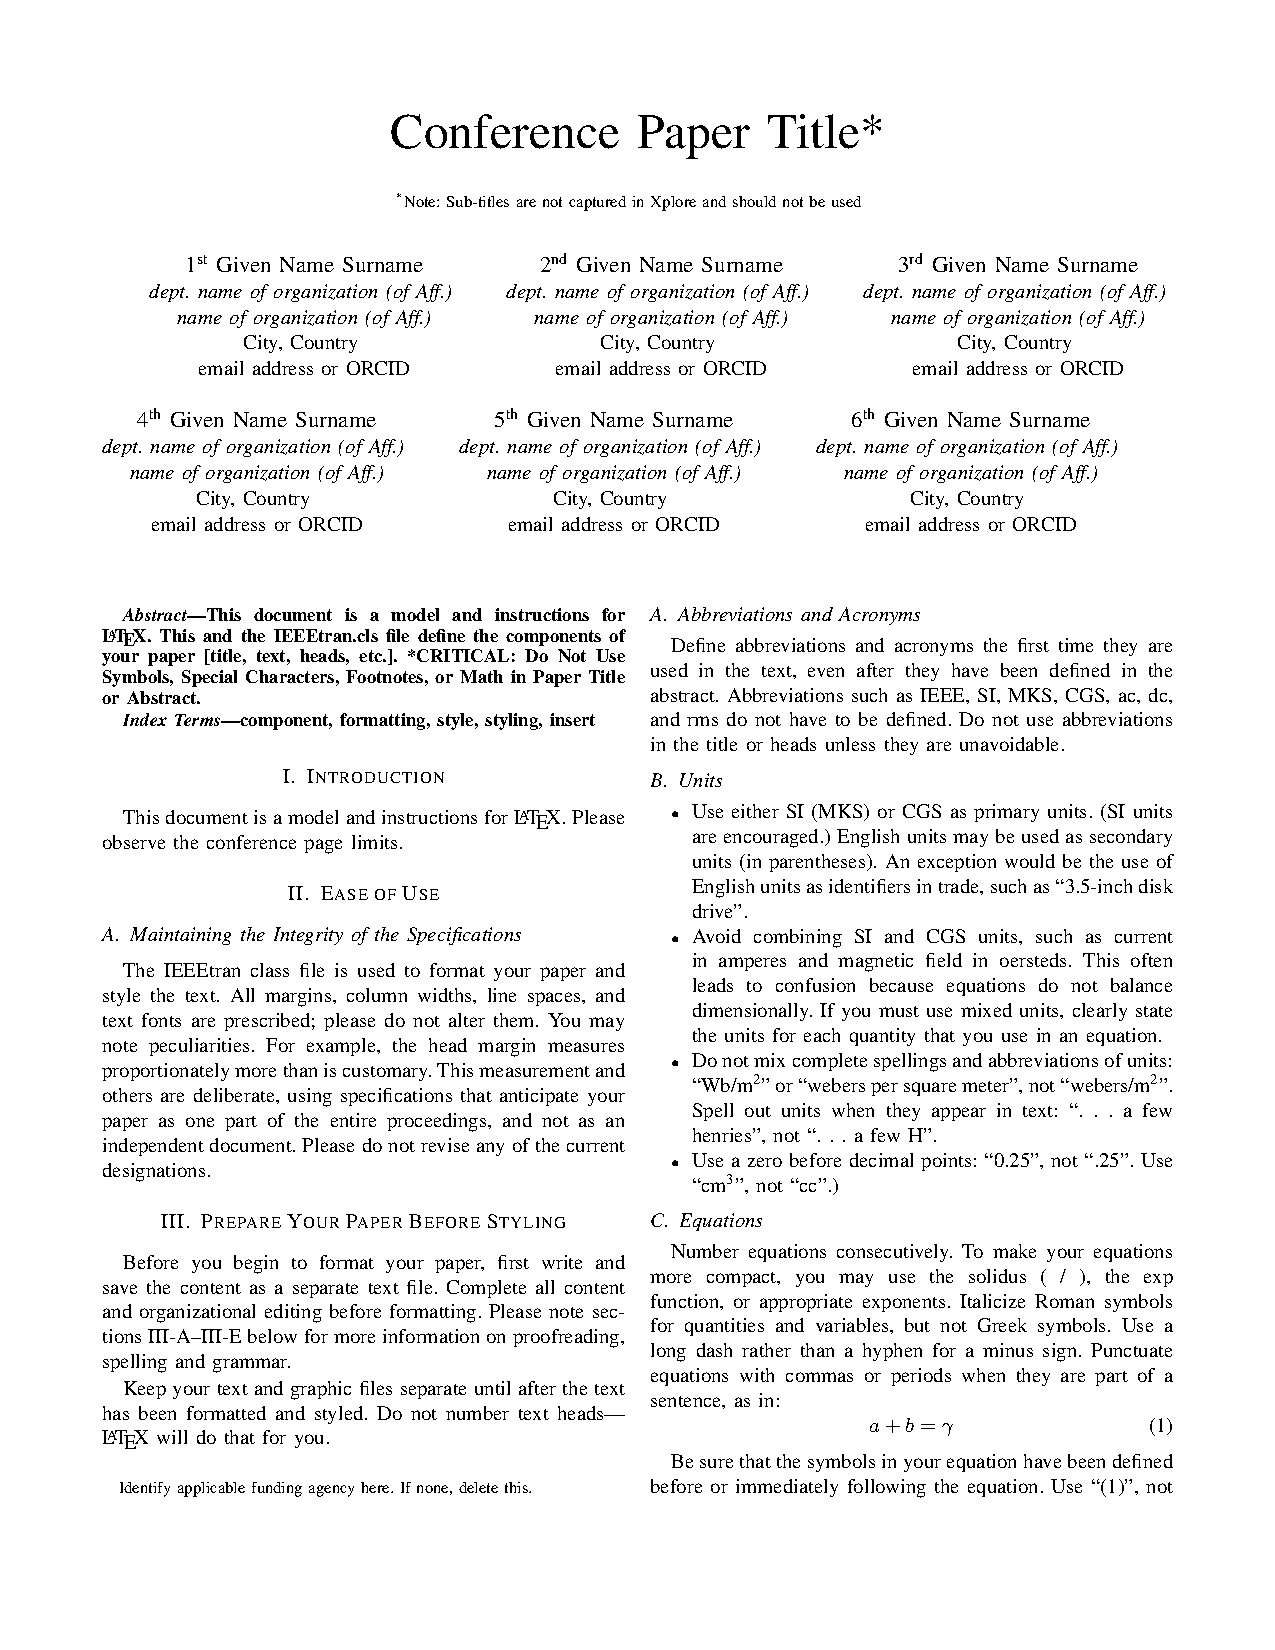
\includepdf[pages=1-3,openright]{PDFs/ieee-conference-template}

\chapter[Additional material]{Additional material}
\label{extra-material}
\include{sections/11_Appendices}

\chapter[Poster]{Poster}
%\includepdf[pages=1,openright]{PDFs/Poster}

\end{document}

%%% Local Variables:
%%% mode: latex
%%% TeX-master: t
%%% End:
